  %
  %
  %
%+++++++++++++++++++++++++++++++++++++++++++++++++++++++++++++++++++
%    To Do:
%
%
%
%-------------------------------------------------------------------
% OPTIONAL PREAMBLE FOR LOCAL COMPILE  %
  %
 \def\titlename{Traverse Notices}
 \def\authorName{Allegan County GIS Services}
 \def\pdfTitle{Traverse Notices}
 \def\pdfSubject{GIS Tools} %
 \def\pdfKeywords{drains,gis}

 %+++++++++++++++++++++++++++++++++++++++++++++++++++++++++++++++++++
%  Used in Subsections that are capable of being compiled alone
%
%
%-------------------------------------------------------------------
\documentclass[letterpaper, 12pt]{memoir}
 %
\usepackage{import} % Required for importing other .tex docs.  (import uses everything bw Begin and End Doc)
\usepackage{float} % Required for specifying the exact location of a figure or table
\usepackage{graphicx} % Required for including images
\usepackage{wrapfig}
\usepackage[pdftex,breaklinks,colorlinks=true,linkcolor=black,citecolor=blue,urlcolor=red,linktocpage=false,pagebackref=true,filecolor=magenta]{hyperref}%http://www.tug.org/applications/hyperref/manual.html#x1-100003.6
\usepackage{cite}
\usepackage[toc,title,page]{appendix}
\usepackage{pdfpages} % enables loading a pdf into the doc
\usepackage{makeidx}
\usepackage{glossaries} % must be after hyperref
\usepackage{blindtext}
\usepackage{enumitem}
%\usepackage{caption}

%\setlist[description]{leftmargin=\parindent,labelindent=\parindent}

%\renewcommand*{\bibname}{References} % renames the bibliography

\newcommand{\HRule}{\rule{\linewidth}{0.5mm}} % Command to make the lines in the title page

\graphicspath{{img/}{GIS_ChampionSection/img/}{awardsChapter/GIS_ChampionSection/img/}{brandPart/awardsChapter/GIS_ChampionSection/img/}{img/}{pairedProgSection/img/}{methodChapter/pairedProgSection/img/}{methodPart/methodChapter/pairedProgSection/img/}{documentationSection/img/}{methodChapter/documentationSection/img/}{methodPart/methodChapter/documentationSection/img/}{docStorageOrgSection/img/}{methodChapter/docStorageOrgSection/img/}{methodPart/methodChapter/docStorageOrgSection/img/}{QGisSection/img/}{toolsChapter/QGisSection/img/}{servicePart/toolsChapter/QGisSection/img/}{ESRISection/img/}{toolChapter/ESRISection/img/}{servicePart/toolChapter/ESRISection/img/}{../../../../source/}{../../source/}{servicePart/applicationsChapter/treasurerSection/img/}}

%\setlength\parindent{0pt} % eliminates indents

 %
%
%%%%%%%%%%%%%%%%%%%%%%%%%%%%%%%%%%%%%%%%%%%%%%%%%%%%%%%%%%%%%%
\graphicspath{{img/}{GIS_ChampionSection/img/}{awardsChapter/GIS_ChampionSection/img/}{brandPart/awardsChapter/GIS_ChampionSection/img/}{img/}{pairedProgSection/img/}{methodChapter/pairedProgSection/img/}{methodPart/methodChapter/pairedProgSection/img/}{documentationSection/img/}{methodChapter/documentationSection/img/}{methodPart/methodChapter/documentationSection/img/}{docStorageOrgSection/img/}{methodChapter/docStorageOrgSection/img/}{methodPart/methodChapter/docStorageOrgSection/img/}{QGisSection/img/}{toolsChapter/QGisSection/img/}{servicePart/toolsChapter/QGisSection/img/}{ESRISection/img/}{toolChapter/ESRISection/img/}{servicePart/toolChapter/ESRISection/img/}{../../../../source/}{../../source/}{servicePart/applicationsChapter/treasurerSection/img/}{servicePart/toolsChapter/gisAdminSection/img/}{gisAdminSection/img/}{servicePart/toolsChapter/bsaSupportSection/img/}{servicePart/toolsChapter/coreDataEditsSection/img/}{servicePart/toolsChapter/coreDataSchemaSection/img/}{../img}{servicePart/applicationsChapter/equalizationSection/img/}{servicePart/toolsChapter/pythonScriptsSection/img/}{servicePart/toolsChapter/ESRISection/img/}{servicePart/applicationsChapter/drainsSection/img/}}


%C:\AC\jalapeno\processing\servicePart\applicationsChapter\drainsSection\img

 %
%   This script does not require Memoir Class
%%%%%%%%%%%%%%%%%%%%%%%%%%%%%%%%%%%%%%%%%%%%%%%%%%%%%%%%%%%%
%+++++++++++++++++++++++++++++++++++++++++++++++++++++++++++++++++++
% Custom Color pallette
    % Blues
\definecolor{HeaderBlueA}{RGB}{85,125,161}
\definecolor{HeaderBlueB}{RGB}{53, 98, 138}
\definecolor{HeaderBlueC}{RGB}{31,78,121}  % HeaderBlue1
\definecolor{HeaderBlueD}{RGB}{16, 60, 99}
\definecolor{HeaderBlueE}{RGB}{4, 40, 72 }
    % Oranges
\definecolor{HeaderOrangeA}{RGB}{249, 161, 121}
\definecolor{HeaderOrangeB}{RGB}{214, 116, 72}
\definecolor{HeaderOrangeC}{RGB}{187, 84, 37}
\definecolor{HeaderOrangeD}{RGB}{152, 57, 14}
\definecolor{HeaderOrangeE}{RGB}{111, 35, 0}
    % Golds
\definecolor{HeaderGoldA}{RGB}{249, 218, 121}
\definecolor{HeaderGoldB}{RGB}{214, 180, 72}
\definecolor{HeaderGoldC}{RGB}{187, 151, 37}
\definecolor{HeaderGoldD}{RGB}{152, 119, 14}
\definecolor{HeaderGoldE}{RGB}{111, 84, 0}
    % Greens
    % option 1
% \definecolor{HeaderGreenA}{RGB}{14, 219, 76}
% \definecolor{HeaderGreenB}{RGB}{23, 179, 70}
% \definecolor{HeaderGreenC}{RGB}{31, 131, 61}
% \definecolor{HeaderGreenD}{RGB}{30, 92, 49}
% \definecolor{HeaderGreenE}{RGB}{21, 50, 30}
    % option 2 (triad of HeaderBlueC)
\definecolor{HeaderGreenA}{RGB}{82, 169, 136}
\definecolor{HeaderGreenB}{RGB}{49, 145, 109}
\definecolor{HeaderGreenC}{RGB}{25, 126, 88}
\definecolor{HeaderGreenD}{RGB}{10, 103, 68}
\definecolor{HeaderGreenE}{RGB}{0, 75, 47}
% Color triad based on HeaderBlue1
% http://paletton.com/

\definecolor{HyperlinkBlue1}{RGB}{64,172,209}
\definecolor{graphicOrange}{RGB}{255,153,51}
\definecolor{gisRed}{RGB}{244,66,66}
%-------------------------------------------------------------------

 %
%%%%%%%%%%%%%%%%%%%%%%%%%%%%%%%%%%%%%%%%%%%%%%%%%%%%%%%%%%%%%%%%%%%%%%%%%%%%
    % Sets sectioning Layout Properties
    %
    %
    %\setsecnumdepth{subsection} % turns on subsec numbering
    %
\setsecheadstyle{\scshape\color{HeaderOrangeA}} % default is \Large\bfseries
    %\setsecheadstyle{\scshape\color{HeaderOrangeB}}
    %
    % Subsection
\setsubsecheadstyle{\large\scshape\color{HeaderOrangeB}} % default is \large\bfseries
    %\setsubsecheadstyle{\huge\centering\color{HeaderOrangeE}}%
    % Subsubsection
\setsubsubsecheadstyle{\Huge\scshape\centering\color{HeaderBlueE}} % default is \bfseries
    %\setsubsubsecheadstyle{\LARGE\scshape\centering\color{HeaderBlueC}}%   1
    % Paragraph
\setparaheadstyle{\bfseries\Large\color{HeaderBlueC}}%
     %\setparaheadstyle{\Large\color{HeaderBlueA}}%2
     % Subparagraph
     %\setsubparaheadstyle{\large\color{HeaderBlueB}}%
\setsubparaheadstyle{\bfseries\large\color{HeaderOrangeB}}%
     %
     % \setbeforeSskip{<skip>} pg .95
     % The absolute value of the <skip> length argument is the space to leave above the heading.
     % If the actual value is negative then the first line after the heading will not be indented.
\setbeforesecskip{-35pt plus -10pt minus -2pt}
\setbeforesubsecskip{-32.5pt plus -10pt minus -2pt}
\setbeforesubsubsecskip{-32.5pt plus -10pt minus -2pt}
\setbeforeparaskip{-32.5pt plus -10pt minus -2pt}
\setbeforesubparaskip{-5pt plus -3pt minus -1pt}
    %
    % \setSindent{<length>}
    % The value of the length argument is the indentation of the heading (number and
    % title) from the lefthand margin. This is normally 0pt.
\setsubparaindent{0pt}
    % \setafterSskip{<skip>} pg.96
    % If the value of the <skip> length argument is positive it is the space to leave between the
    % display heading and the following text. If it is negative, then the heading will be runin
    % and the value is the horizontal space between the end of the heading and the following text.
    %
\setaftersecskip{.05in}
\setaftersubsecskip{.15in}
\setaftersubsubsecskip{.1in}
\setafterparaskip{.05in}
\setaftersubparaskip{.05in}
    %
\renewcommand{\partnamefont}{\color{HeaderOrangeE}\Huge\normalfont}
\renewcommand{\partnumfont}{\color{HeaderOrangeE}\Huge\normalfont}
    %
    % End of Setting sectioning Layout Properties
%%%%%%%%%%%%%%%%%%%%%%%%%%%%%%%%%%%%%%%%%%%%%%%%%%%%%%%%%%%%%%%%%%%%%%%%%%%%
\setlength\columnsep{.3in}

 %
%%%%%%%%%%%%%%%%%%%%%%%%%%%%%%%%%%%%%%%%%%%%%%%%%%%%%%%%%%%%
% HEADERS AND FOOTERS
%%%%%%%%%%%%%%%%%%%%%%%%%%%%%%%%%%%%%%%%%%%%%%%%%%%%%%%%%%%%
          %This script requires Memoir Class
    %  Page Styles
    %  In LATEX the page style refers to the part of the page building mechanism that
    %   attaches the headers and footers to the actual page.
%%%%%%%%%%%%%%%%%%%%%%%%%%%%%%%%%%%%%%%%%%%%%%%%%%%%%%%%%%%%
%  This block defines jalapenoPageStyleA page style
\makepagestyle{jalapenoPageStyleA}
    % headers
\makeheadrule {jalapenoPageStyleA}{\textwidth}{\normalrulethickness}
\makeheadfootruleprefix{jalapenoPageStyleA}{\color{HeaderOrangeE}}{\color{HeaderOrangeE}}
\makeevenhead {jalapenoPageStyleA}{\helv \thepage}{} {\helv \rightmark}
\makeoddhead {jalapenoPageStyleA}{\helv \leftmark}{}{\helv \thepage}
    % footers
\makefootrule {jalapenoPageStyleA}{\textwidth}{\normalrulethickness}{\footruleskip}
\makeevenfoot {jalapenoPageStyleA}{}{} {}
\makeoddfoot {jalapenoPageStyleA}{}{} {}
    %
%%%%%%%%%%
    %
%  This block defines marks for jalapenoPageStyleA page style
    %  See page 11 of Page Styles in Memoir
    %
\makeatletter % because of \@chapapp
%
\makepsmarks {jalapenoPageStyleA}{
%\nouppercaseheads
\createmark {chapter} {both} {shownumber}{\@chapapp\ }{. \ } % set leftmark to chapter
%\createmark {section} {right}{shownumber}{} {. \ }
\createmark {subsection} {right}{shownumber}{} {. \ } % set rightmark to subsection
%\createmark {subsubsection}{right}{shownumber}{} {. \ } % set rightmark to subsubsection
\createplainmark {toc} {both} {\contentsname}
\createplainmark {lof} {both} {\listfigurename}
\createplainmark {lot} {both} {\listtablename}
\createplainmark {bib} {both} {\bibname}
\createplainmark {index} {both} {\indexname}
\createplainmark {glossary} {both} {\glossaryname}

}
\makeatother
%  End of jalapenoPageStyleA pagestyle
%%%%%%%%%%%%%%%%%%%%%%%%%%%%%%%%%%%%%%%%%%%%%%%%%%%%%%%%%%%%

%%%%%%%%%%%%%%%%%%%%%%%%%%%%%%%%%%%%%%%%%%%%%%%%%%%%%%%%%%%%
%  This block defines emptyPageStyle page style
\makepagestyle{emptyPageStyle}
    % headers
\makeevenhead {emptyPageStyle}{}{}{}
\makeoddhead {emptyPageStyle}{}{}{}
    % footers
\makefootrule {emptyPageStyle}{}{}{}
\makeevenfoot {emptyPageStyle}{}{}{}
\makeoddfoot {emptyPageStyle}{}{}{}
    %
%%%%%%%%%%
\newcommand{\normPageLayout}{%
\setmarginnotes{.2in}{.5in}{.1in}%
\setlrmarginsandblock{*}{0.3\paperwidth}{.75}% Left right ratio
\setulmarginsandblock{1in}{*}{*}%
\checkandfixthelayout%
\clearpage}

\newcommand{\widePageLayout}{%
\setmarginnotes{.1mm}{.1mm}{.1mm}%
\setlrmarginsandblock{1in}{1in}{*}% Left right ratio
\setulmarginsandblock{1in}{1in}{*}%
\checkandfixthelayout%
\clearpage}

 %
%%%%%%%%%%%%%%%%%%%%%%%%%%%%%%%%%%%%%%%%%%%%%%%%%%%%%%%%%%%%%%%%%%%%%%%%%%%%
  % beginning od customchpstyle
    %
\makeatletter % handler for @
    %
\makechapterstyle{jalapenoChapterStyle}{%
    %
    \newlength{\chapColorbarheight}
    \setlength{\chapColorbarheight}{.06in}		% Setting the height of the bar
    %
    \newlength{\chapnumboxlength}
    \setlength{\chapnumboxlength}{.75in}	% Setting the length of the box containing chapter number
    %
    \newlength{\leftbarlength}
    \setlength{\leftbarlength}{.5in}  		% Setting length of the bar left to the chapter number
    \setlength{\afterchapskip}{.5in}
    \renewcommand*{\chapterheadstart}{\vspace*{.25in}} % vspace from top of page
    \renewcommand*{\afterchapternum}{\vspace*{-.9in}} % neg moves chapter title above chapter number
    \renewcommand*{\chapnumfont}{\slshape} % Number Font
    \renewcommand*{\chaptitlefont}{\flushright\color{HeaderOrangeE}\slshape\huge}
    \renewcommand*{\printchaptername}{} % sets the text in brackets before the number
    %\makeatletter
    \newcommand*{\thickrulefill}{\leavevmode \leaders \hrule height \chapColorbarheight \hfill \kern \z@} % rightbar length setter
    %\makeatother
    \renewcommand*{\printchapternum}{%
        %\makebox[0pt][l]{%
        \color{HeaderOrangeE}
        \rule{\leftbarlength}{\chapColorbarheight} % Left bar
        \quad % hspace
        \resizebox{!}{\chapnumboxlength}
        {\chapnumfont \thechapter} % Chapter name and number
        \quad % hspace
        \color{HeaderOrangeE}\thickrulefill % implements thickrulefill
     } %
     \makeatother % closes handler for @
} % End of customchpstyle
%%%%%%%%%%%%%%%%%%%%%%%%%%%%%%%%%%%%%%%%%%%%%%%%%%%%%%%%%%%%%%%%%%%%%%%%%%%%

 %
%\newglossaryentry{ex}{name={sample},description={an example}}


\newglossaryentry{projection}{name={map projection},description={Representing a sphere on a flat surface}}
 %
\newlength\drop
\makeatletter
\newcommand*\titleM{\begingroup% Misericords, T&H p 153
\setlength\drop{0.08\textheight}
\centering
\vspace*{\drop}
{\protect\HRule}
\begin{figure}[H] % included image
\begin{center}	% centered horizontally
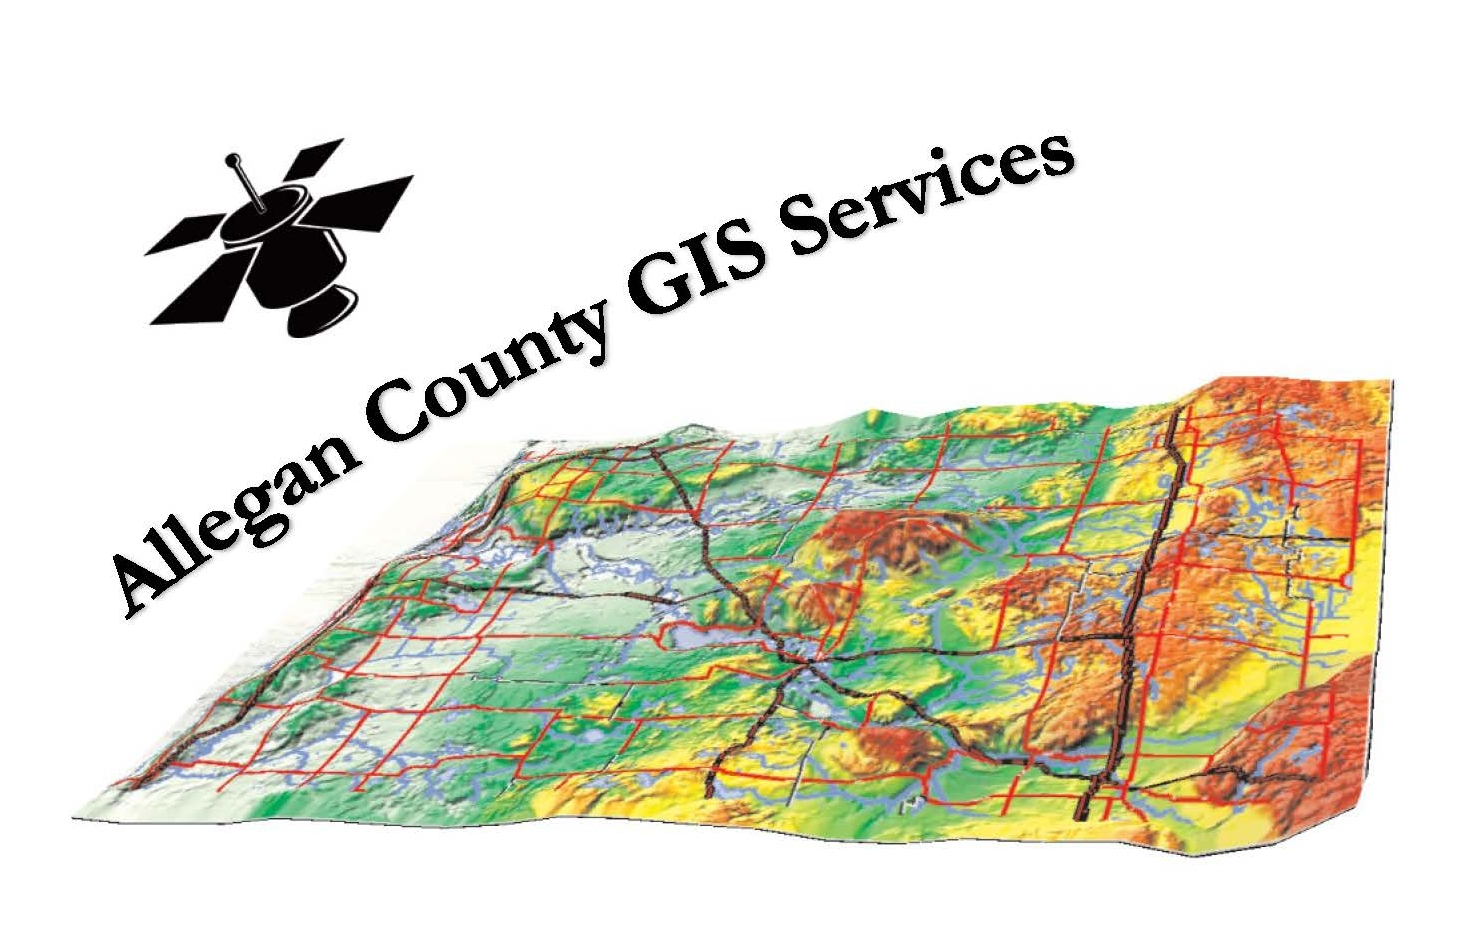
\includegraphics[scale=.5]{GIS_Logo_better.jpg}
\end{center}
\end{figure}
\vspace{-.1in}
{\Huge\bfseries\titlename}\\[2\baselineskip]
{\protect\HRule}\\[\baselineskip]
{\small\scshape www.allegancounty.org/gis}\\[2\baselineskip]
{\small\scshape \@date}\par
\endgroup}
\makeatother
  % inputs common title
  % SET PDF METADATA  %
\hypersetup{pdfauthor={\authorName},
pdftitle={\pdfTitle}, %  Sets PDF properties
pdfsubject={\pdfSubject},
pdfkeywords={\pdfKeywords}}
%-------------------------------------------------------------------
  % TOC DEPTH  %
\setcounter{tocdepth}{5}  % Sets Table of Contents level to show
                             % subparagraphs(5), paragraphs(4),
                             % subsubsections(3), subsections(2(default)),
                             % sections(1), chapters and parts(0)
 %
%+++++++++++++++++++++++++++++++++++++++++++++++++++++++++++++++++++
%    SET TEXT BLOCK AND MARGINS FOR COVER PAGE  %
\setmarginnotes{.1in}{.4in}{.1in}
\setlrmarginsandblock{*}{0.18\paperwidth}{1} % Left right ratio
\setulmarginsandblock{1in}{1in}{*}
\checkandfixthelayout
\makeatletter
\ch@ngetext
\makeatother
  %+++++++++++++++++++++++++++++++++++++++++++++++++++++++++++++++++++
	%  Front Section
  %-------------------------------------------------------------------
\begin{document}% document begins
   %
\frontmatter % turns off chapter numbering and uses roman numerals for page numbers
   %
\pagestyle{plain}
   %
\begin{titlingpage}
   %
\titleM  % Inputs titleM
   %
\end{titlingpage}
   %
%+++++++++++++++++++++++++++++++++++++++++++++++++++++++++++++++++++
%    SET TEXT BLOCK AND MARGINS FOR MAIN DOCUMENT PAGES   %
\setmarginnotes{.1in}{.4in}{.1in}
\setlrmarginsandblock{*}{0.18\paperwidth}{.75} % Left right ratio
\setulmarginsandblock{1in}{1in}{*}
\checkandfixthelayout
\makeatletter
\ch@ngetext
\makeatother
%-------------------------------------------------------------------
\tableofcontents % creates TOC
  %
%+++++++++++++++++++++++++++++++++++++++++++++++++++++++++++++++++++
%		Main Section
%-------------------------------------------------------------------
\mainmatter % turns on chapter numbering, resets page numbering and uses arabic numerals for page numbers
  %
\chapterstyle{jalapenoChapterStyle} % custom from chapterStyles.tex
  %
\pagestyle{jalapenoPageStyleA} % custom from pageStyles.tex

  %
%-------------------------------------------------------------------
    %
    %
%\begin{document}% document begins
 %
 %--------------------------------------------------
\subsection{Traverse Notices Production}
  %
\subsubsection{Problem and Analysis}
  %
\begin{adjmulticols}{2}{\innerMar}{\outerMar}
  %
\paragraph{Background}
  %
\noindent This tool replaces a mapInfo toolset to produce the different notification documents needed for drain maintenance.
  %
\paragraph{Statement of Problem}
  %
\noindent Drains Department must notify property owners affected by drain maintenance. 
  %
\paragraph{Analysis}
  %
\noindent \textbf{Traverse Notification Workflow} will facilitate: generation of notification documents based on a drain selected in a map.  From a selected drain this workflow selects affected parcels and assembles letters and lists with needed information.
  %
\subparagraph{People Involved in the Workflow}
  %
\begin{itemize} %
\item GIS Analyst
\item Drains Staff
\end{itemize} %
  %
\subparagraph*{Stages of the Workflow}
  %
\begin{itemize} %
\item Use the Traverse Notices Letter Task
\item Create a Map
\item Export reports for parcels intersecting selected drains
\end{itemize} %
  %
\end{adjmulticols}
  %
\clearpage
  %
  %
\paragraph{Traverse Notices Workflow Summary}
\vspace{.25in}

The {\LARGE Three Stages} of the workflow \textit{in ArGIS Pro}:

\begin{enumerate}
\item Traverse Notices Letter Task
  %
\begin{itemize}

\item Search for drain
\item Select drain
\item Process data for selected drain

\end{itemize}

\item Create Maps 
\begin{itemize}
\item Set area and zoom level of map
\item Markup map as desired
\item Export map to PDF
\end{itemize}
  %
\item Export Letters
  %
\begin{itemize} %
\item Export individual reports from the Export Report Pane to PDF
\end{itemize} %
\end{enumerate}
  %
\clearpage
  %
  
\paragraph{Technologies Used in The Workflow}
  %
\subparagraph{ArcGIS Pro}
  %
\begin{itemize}
\item SQL Server Source Data(ACPro.SDE)

\item An ArcGIS Pro Task is used to execute geoprocessing 

\item Map creation in ArcGIS Pro

\item Report creation(letters) in ArcGIS Pro

  %
\end{itemize}
   %
   
\subparagraph{Other Software}

\begin{itemize}

\item PDF document printer

\end{itemize}

\subparagraph{Hardware}

\begin{itemize}

\item Printer

\end{itemize}

\clearpage


\subsubsection{Running the task}


\paragraph{Open ArcGISPro}

\begin{itemize}

\item Navigate to: \begin{verbatim}J:\Departments\Drains\Apps\TraverseNotices\Processing\end{verbatim}

\item Click the Project: \textbf{TraverseNoticesTool.aprx}
\begin{figure}[h!]
 \centering
     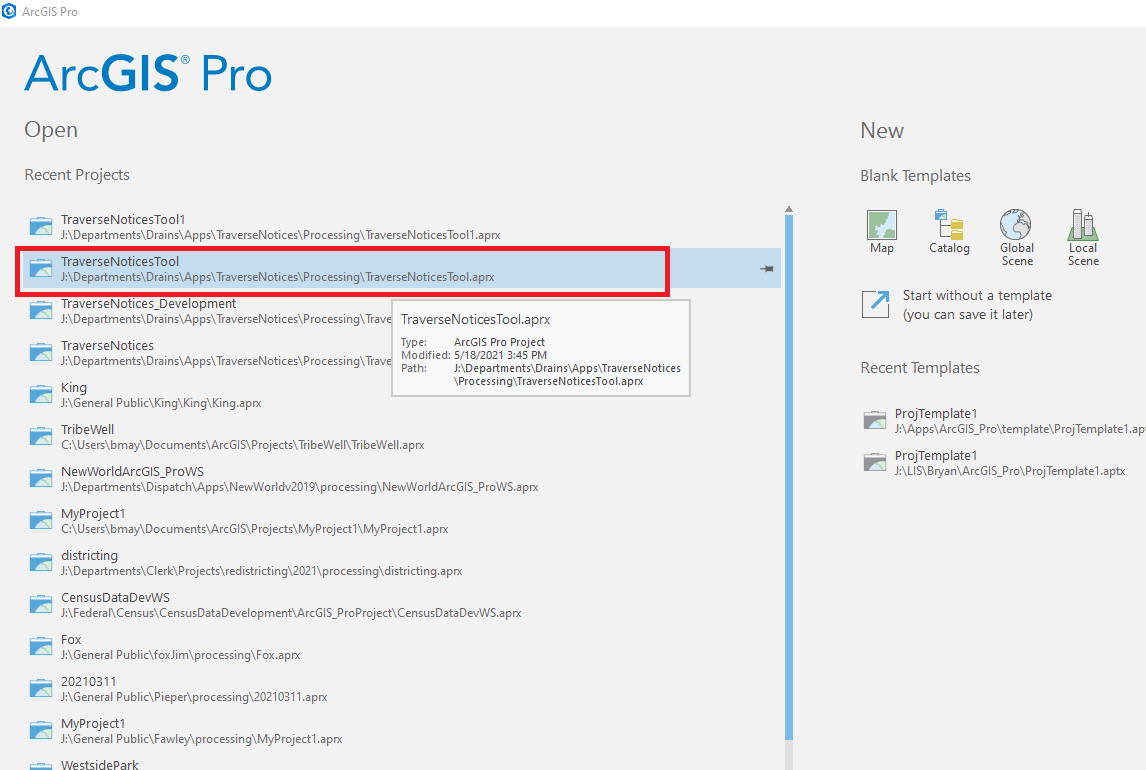
\includegraphics[width=.9\textwidth]{SelectProject1.png}
 \caption{Select Project}
 \end{figure}

\end{itemize}
\clearpage

\paragraph{Workspace Overview}

%\noindent {\btn {Within ArcGisPro: }\fbox{xxx}}
\noindent {\btn {Within ArcGIS Pro:}}

%\subparagraph{Within ArcGisPro:}
\noindent Panes and windows can be placed in any way.\\
\noindent The default layout is depicted below. \\ 
\noindent The important elements for this workflow are:

\begin{itemize}
\item Contents Pane
\item Catalog Pane
\item Tasks Pane
\item Map Pane
\item Attribute Tables
\item Layout Panes
\item Report Panes
\item Geoprocessing Tool Boxes
\end{itemize}

\begin{figure}[h!]
 \centering
     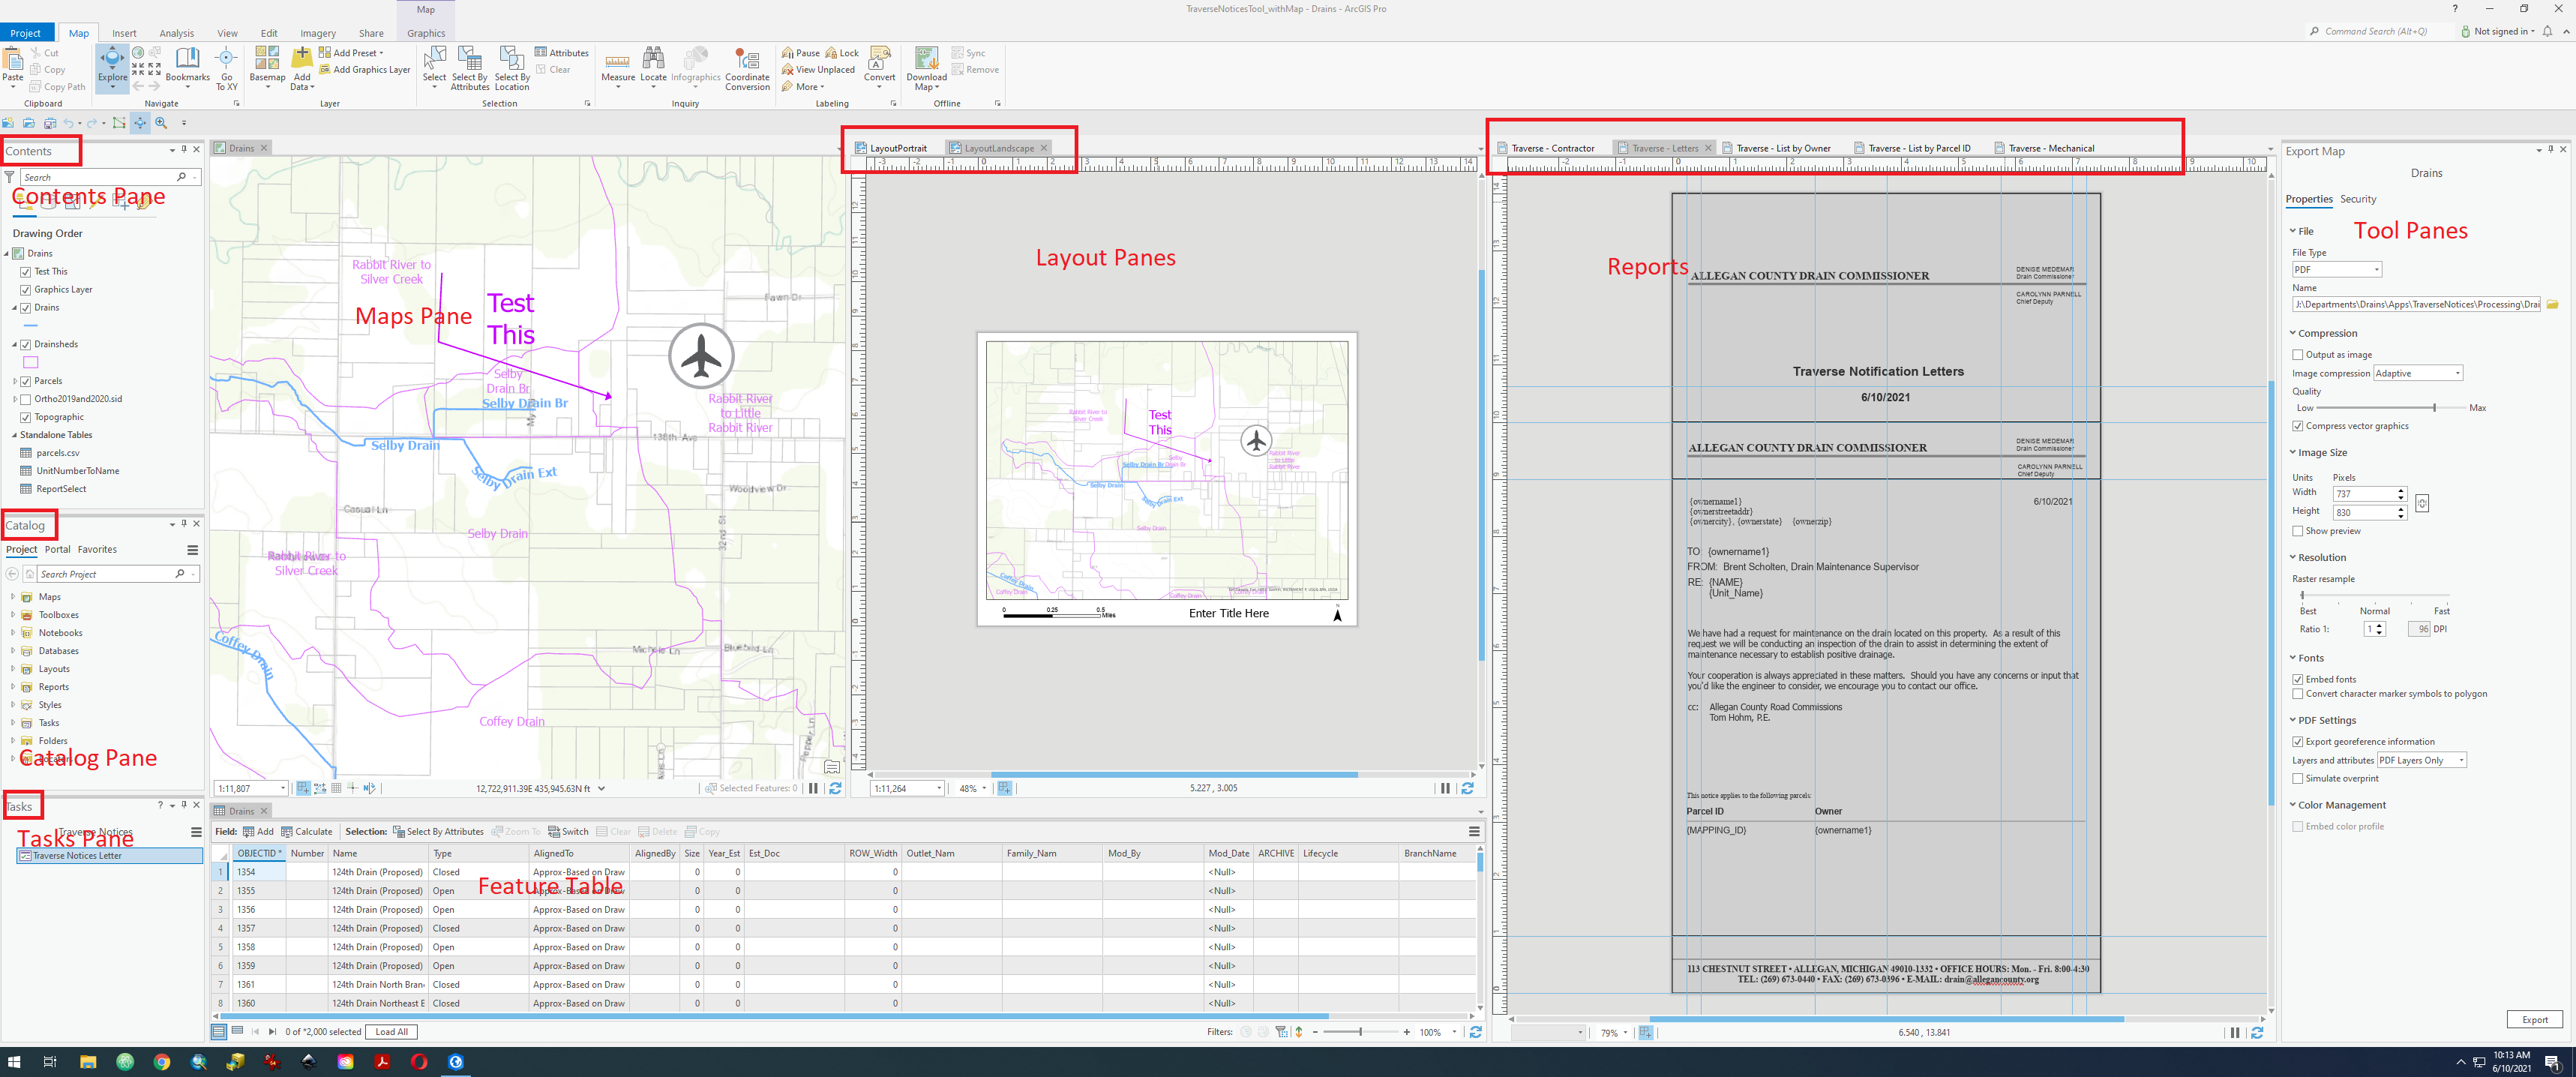
\includegraphics[width=1.2\textwidth]{WS_Desc2.png}
 \caption{Workspace Overview}
 \end{figure}

\clearpage

\paragraph{Begin the Traverse Notices Letter Task}
If needed, click on the the task in catalog and choose {\bigbtn\fbox{Open}}
\begin{itemize}

\item Left click on the task name in Tasks Pane
\item Push green arrow in tasks for Traverse Notices Letter

\end{itemize}
\begin{figure}[h!]
 \centering
     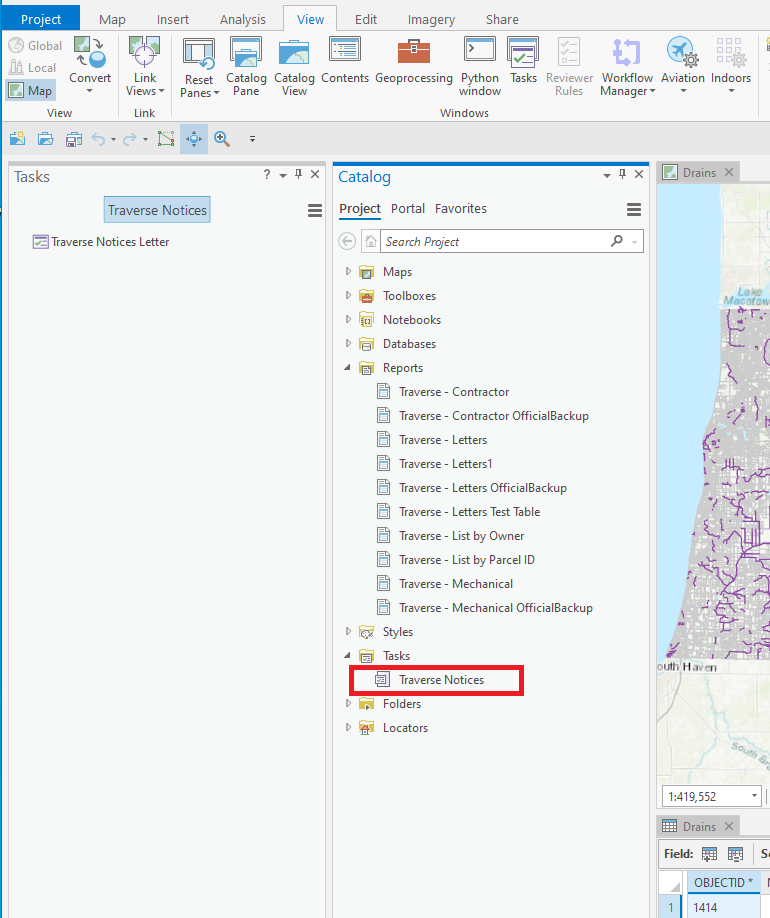
\includegraphics[width=.9\textwidth]{CatalogTour3.png}
 \caption{Open the Task}
 \end{figure}


\clearpage

\paragraph{Search for a drain}

\begin{itemize}

\item In Task Pane, {\bigbtn Click \fbox{Layer Search}} 
\item From dropdown select {\menuArrow}{\bigbtn \fbox{match any part}}
\item Enter partial drain name {\menuArrow}{\bigbtn Push \fbox{enter}}

\end{itemize}

\begin{figure}[h!]
 \centering
     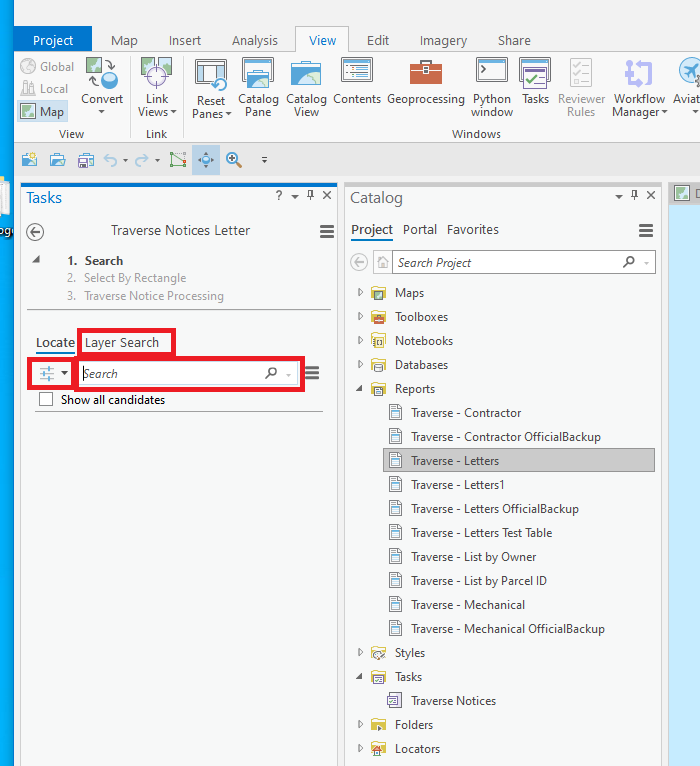
\includegraphics[width=.9\textwidth]{StepOne4a.png}
 \caption{Drain Search}
 \end{figure}

\clearpage

 \begin{wrapfigure}{r}{0.5\textwidth}
 \centering
     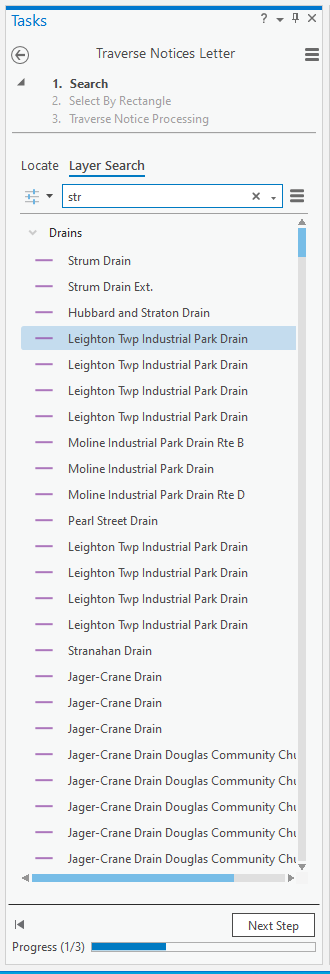
\includegraphics[width=.35\textwidth]{ListOfDrains.png}
 \caption{Drains List}
   \end{wrapfigure}
.

\vspace{1.5in}

\noindent{\bigbtn Right click a drain \lookArrow}
\vspace{.5in}
 
\noindent{\bigbtn \fbox{zoom to selected}\lookArrow}


\clearpage

\subparagraph[Map of Drain]{Navigate the map to the correct area:}

\begin{itemize}

\item Click and hold to pan

\item Use the mouse wheel to zoom in or out

\item Push next step in the task

\end{itemize}

\begin{figure}[h!]
 \centering
     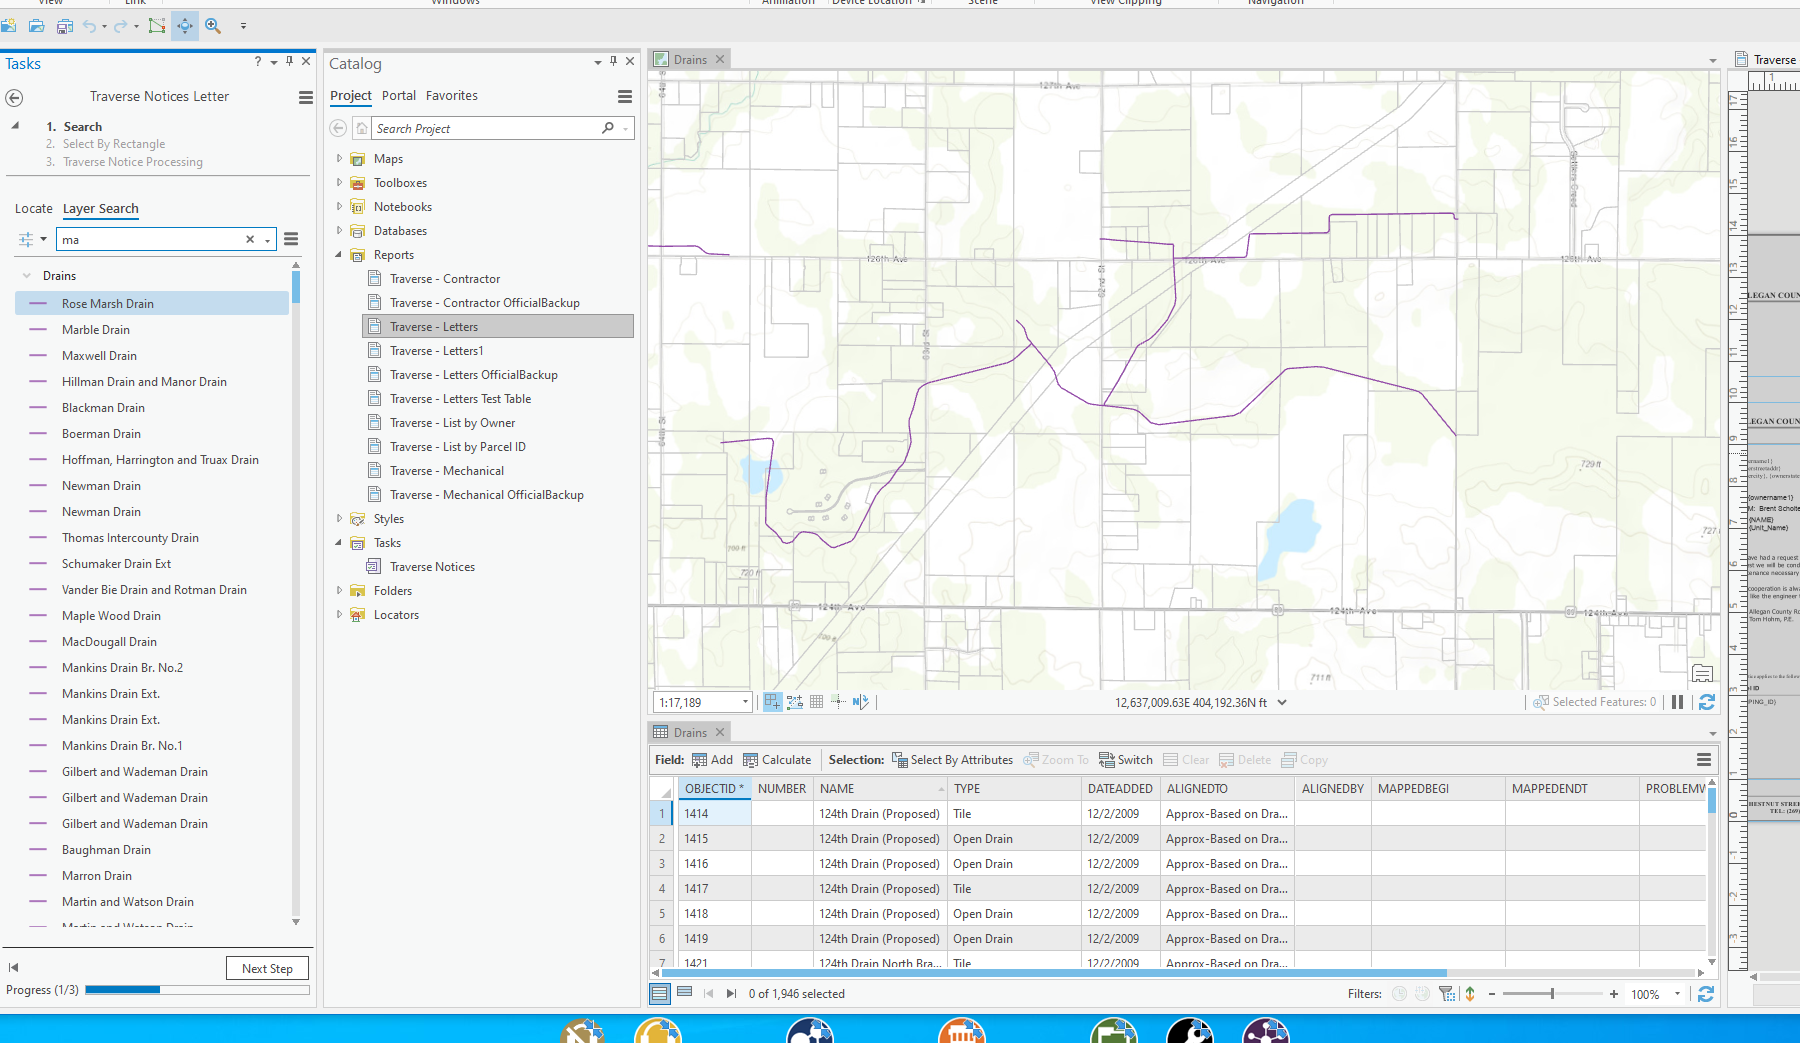
\includegraphics[width=.9\textwidth]{zoomTo7.png}
 \caption{Drain Zoomed}


 \end{figure}

\subparagraph[x]{If the map is in the correct area:}

\begin{itemize}

\item Push \bigbtn \fbox{Next Step}

\end{itemize}

\clearpage

\subparagraph{Select Drains of interest}

\begin{itemize}

\item The select by rectangle tool is enabled

\item Left click and hold to draw a box around the drain

\item To deselect, click away from the selection in the map

\item To add to the selection hold shift and select more drains

\end{itemize}

\begin{figure}[h!]
 \centering
     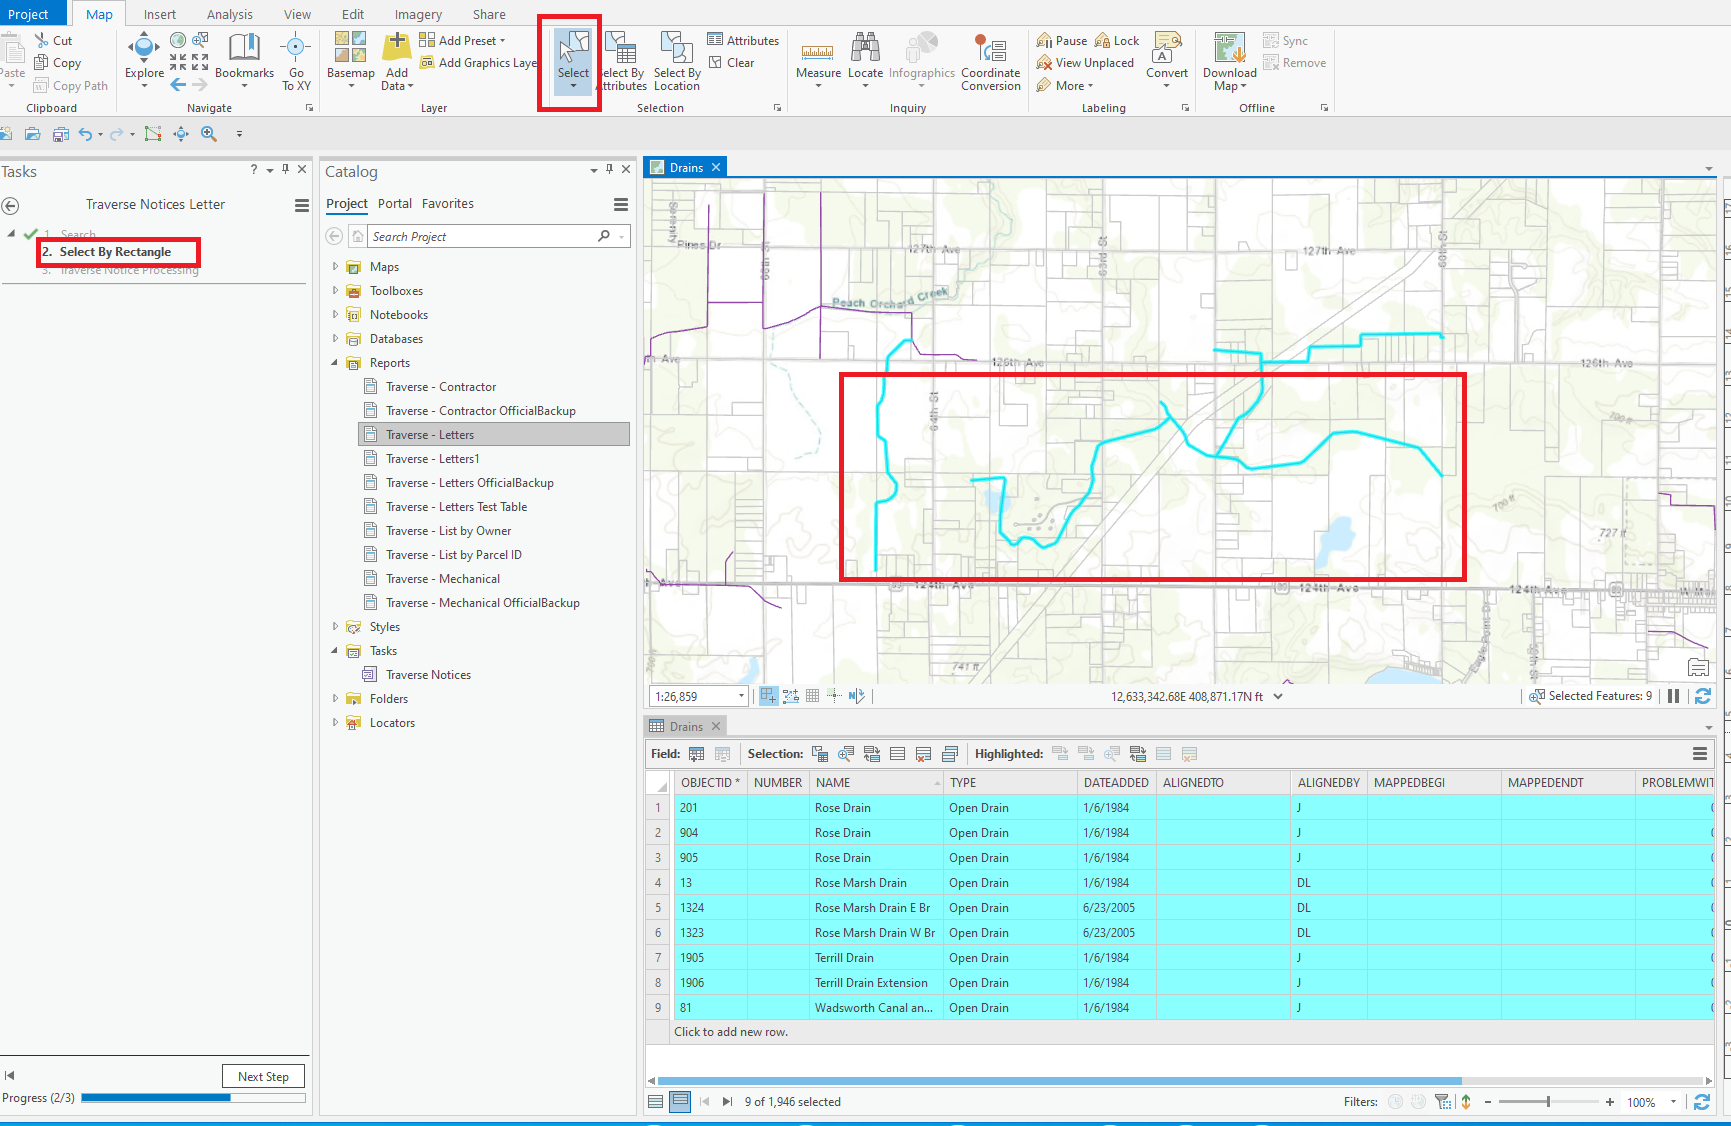
\includegraphics[width=1\textwidth]{drainSelected8.png}
 \caption{Select Drain}


 \end{figure}

\clearpage
     
  
\subparagraph{Highlight Selected Drains}

\noindent To see a list of selected drains:

\begin{itemize}

\item In the Drains table, Push the button for Show selected records

\end{itemize}

\begin{figure}[h!]
 \centering
     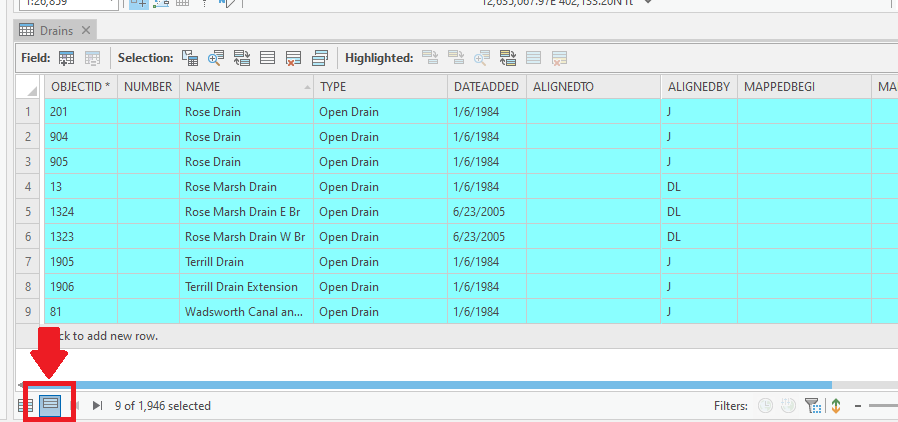
\includegraphics[width=1\textwidth]{showSelectedRecords9.png}
 \caption{Show Selected Drains}


 \end{figure}

\clearpage

\subparagraph{Process Selected Drains}

  \begin{wrapfigure}{r}{0.6\textwidth}
  \centering
      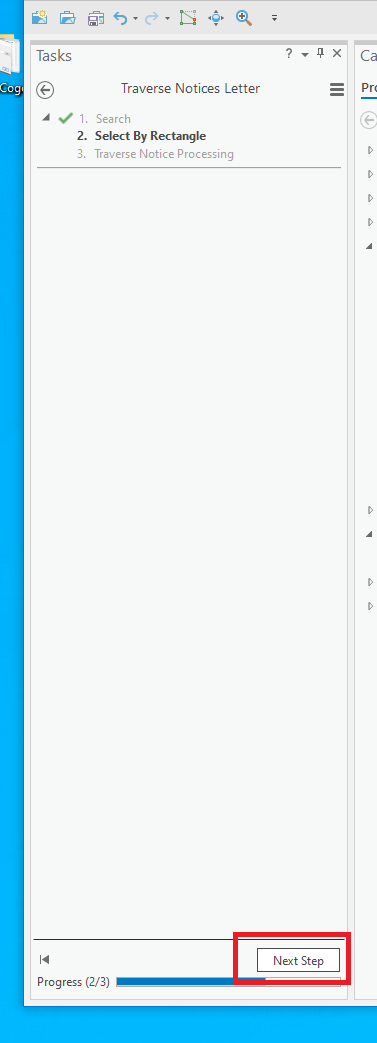
\includegraphics[width=.5\textwidth]{NextStep10.PNG}
  \caption{Process Selected Drains}
  \end{wrapfigure}
.

  \vspace{1.75in}

 \noindent {\btn {Push }\fbox{Next Step}}


\clearpage

\subparagraph{Parcel Selection Process Runs}
\vspace{.5in}

\noindent A selection of parcels is created based on intersection with the selected drains.

\vspace{.5in}

\noindent If the selection of parcels looks correct:

\noindent {\btn {Push }\fbox{Finish}}

\begin{figure}[h!]
 \centering
     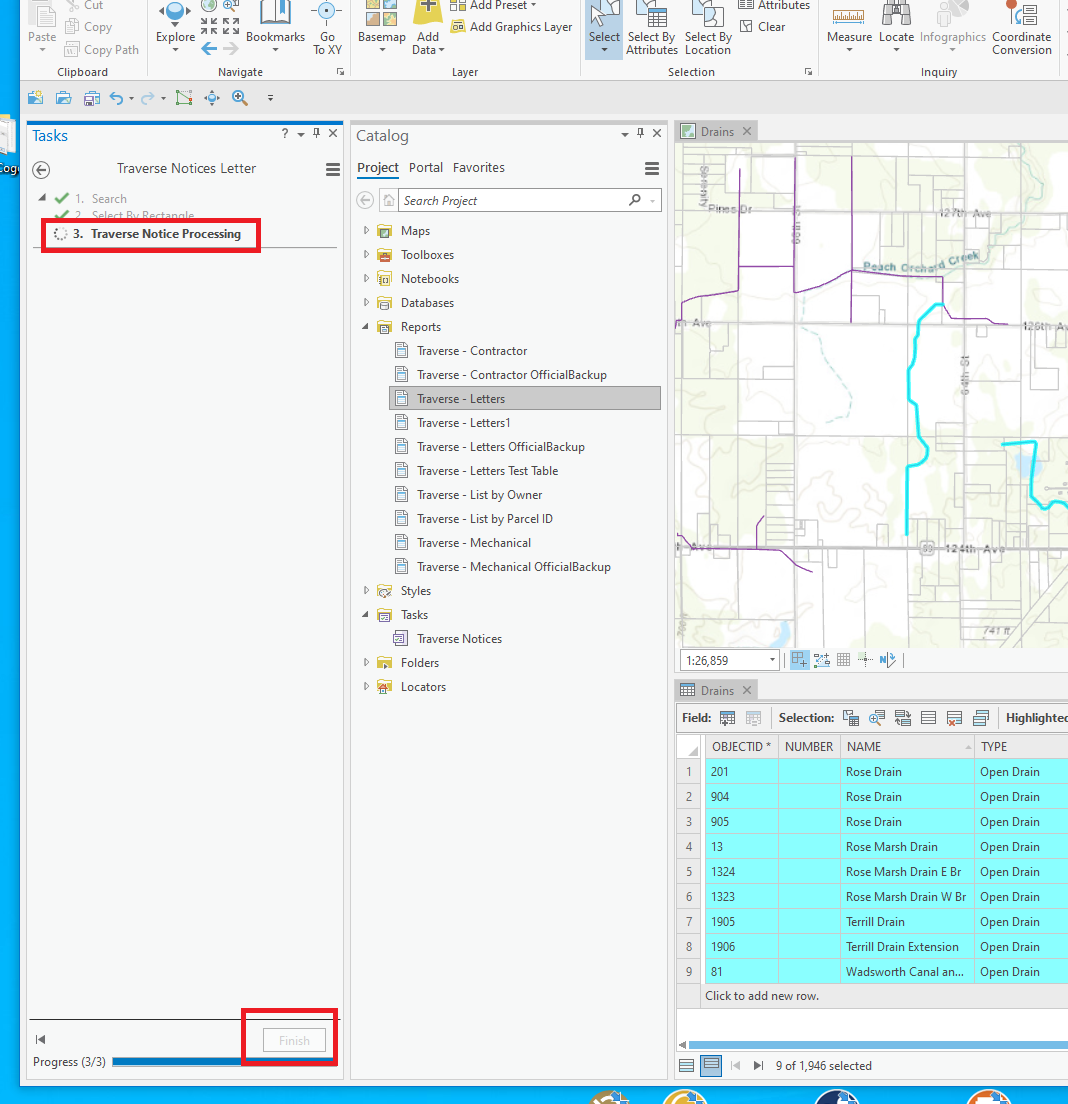
\includegraphics[width=.8\textwidth]{ToolProcesses11.PNG}
 \caption{Traverse Notice Processing}


 \end{figure}
 
\noindent The data is now ready for exporting reports (letters).

\clearpage


\paragraph{Create Reports}

\subparagraph{Select a report to create}
\vspace{.5in}

\noindent Click on tab of desired report

\vspace{1in}

%\noindent {\btn {Push }\fbox{Finish}}

\begin{figure}[h!]
 \centering
     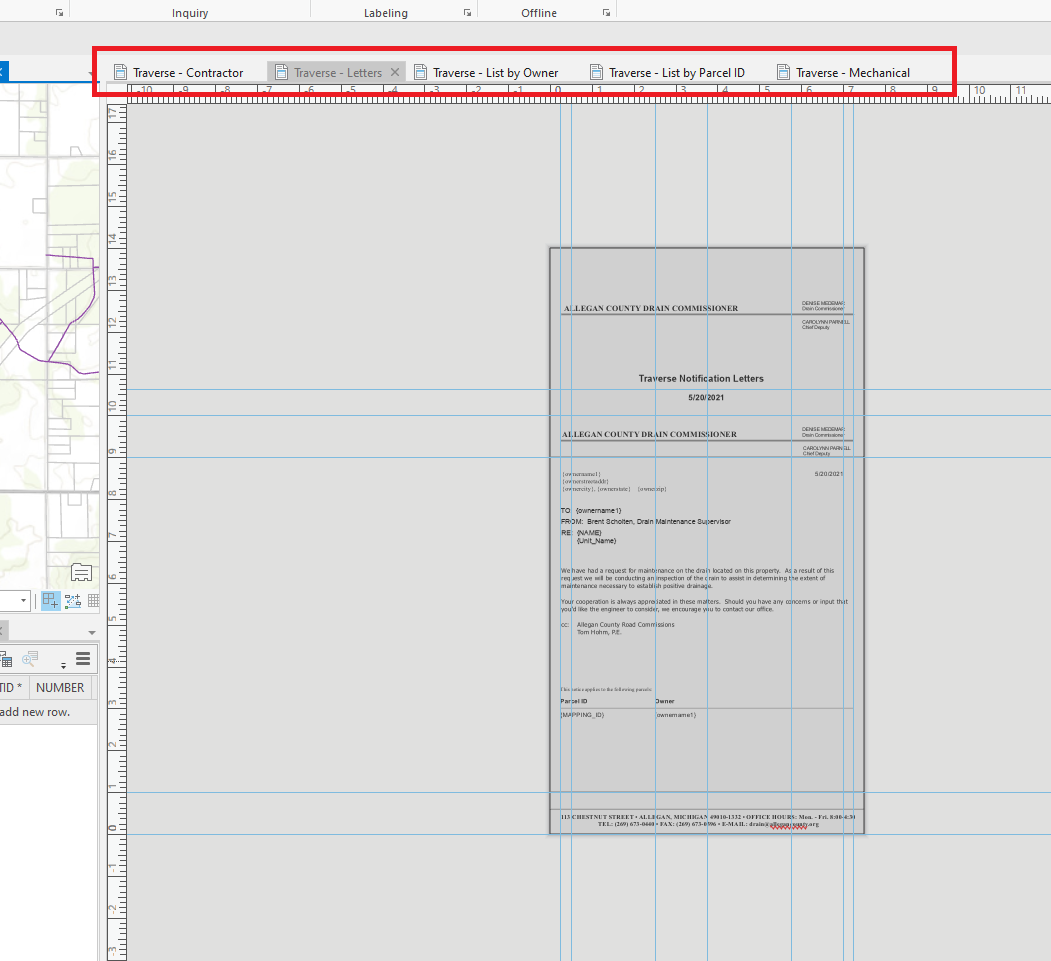
\includegraphics[width=.8\textwidth]{ReportPane12.PNG}
 \caption{Select Report}


 \end{figure}


\clearpage

\subparagraph{Produce the letters}
\vspace{.5in}

\noindent {\btn {Push }\fbox{Export Report} from the Share Tab}

\begin{figure}[h!]
 \centering
     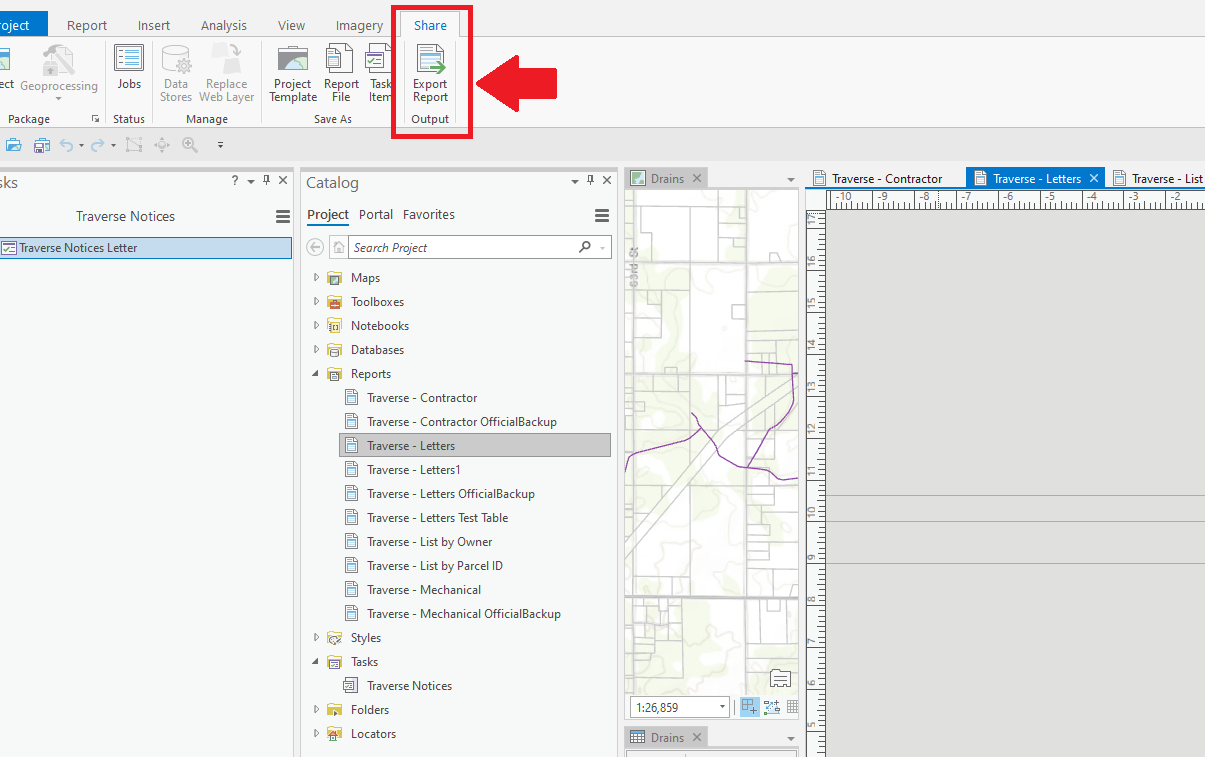
\includegraphics[width=.8\textwidth]{ShareTab13.PNG}
 \caption{Export Report}


 \end{figure} 


\clearpage

\subparagraph{Export Reports}

\begin{itemize}

\item Share each report for all the letters

\item Enter a name and output location for each report

\end{itemize}


\noindent {\btn {Push }\fbox{Export}}

\begin{figure}[h!]
 \centering
     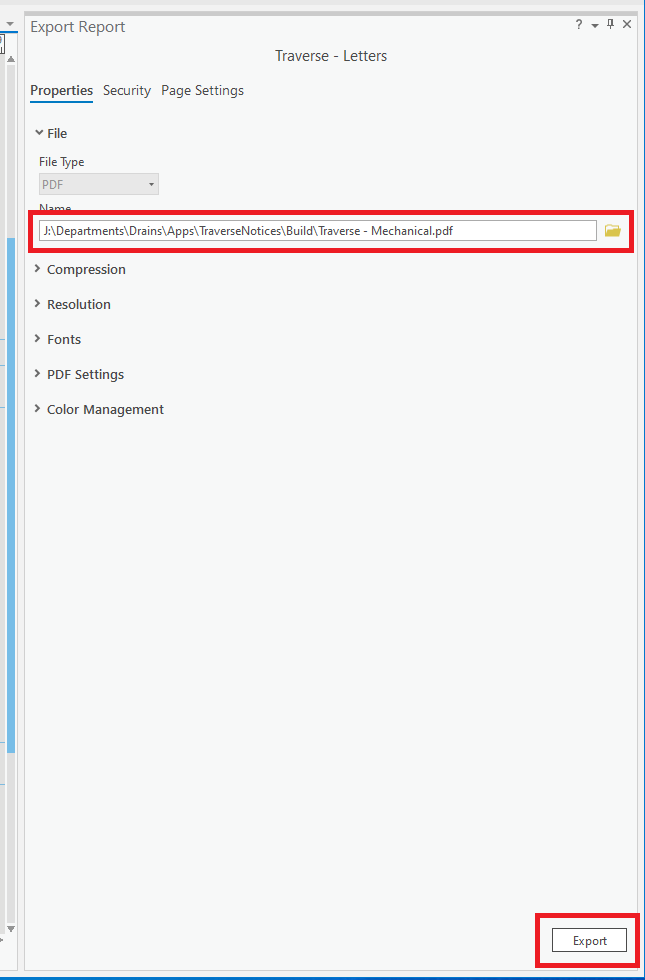
\includegraphics[width=.6\textwidth]{ExportReport14.PNG}
 \caption{Export Report}


 \end{figure} 


\clearpage

\paragraph{Layouts}
Layouts are used to assemble a map document for printing.  To zoom and move around within the layout it must be activated

\subparagraph{Activate Layout Frame}

To activate the Layout Frame:

\vspace{.25in}


\noindent {\btn {Right Click in the Layout and select }\fbox{Activate}}

\begin{figure}[h!]
 \centering
     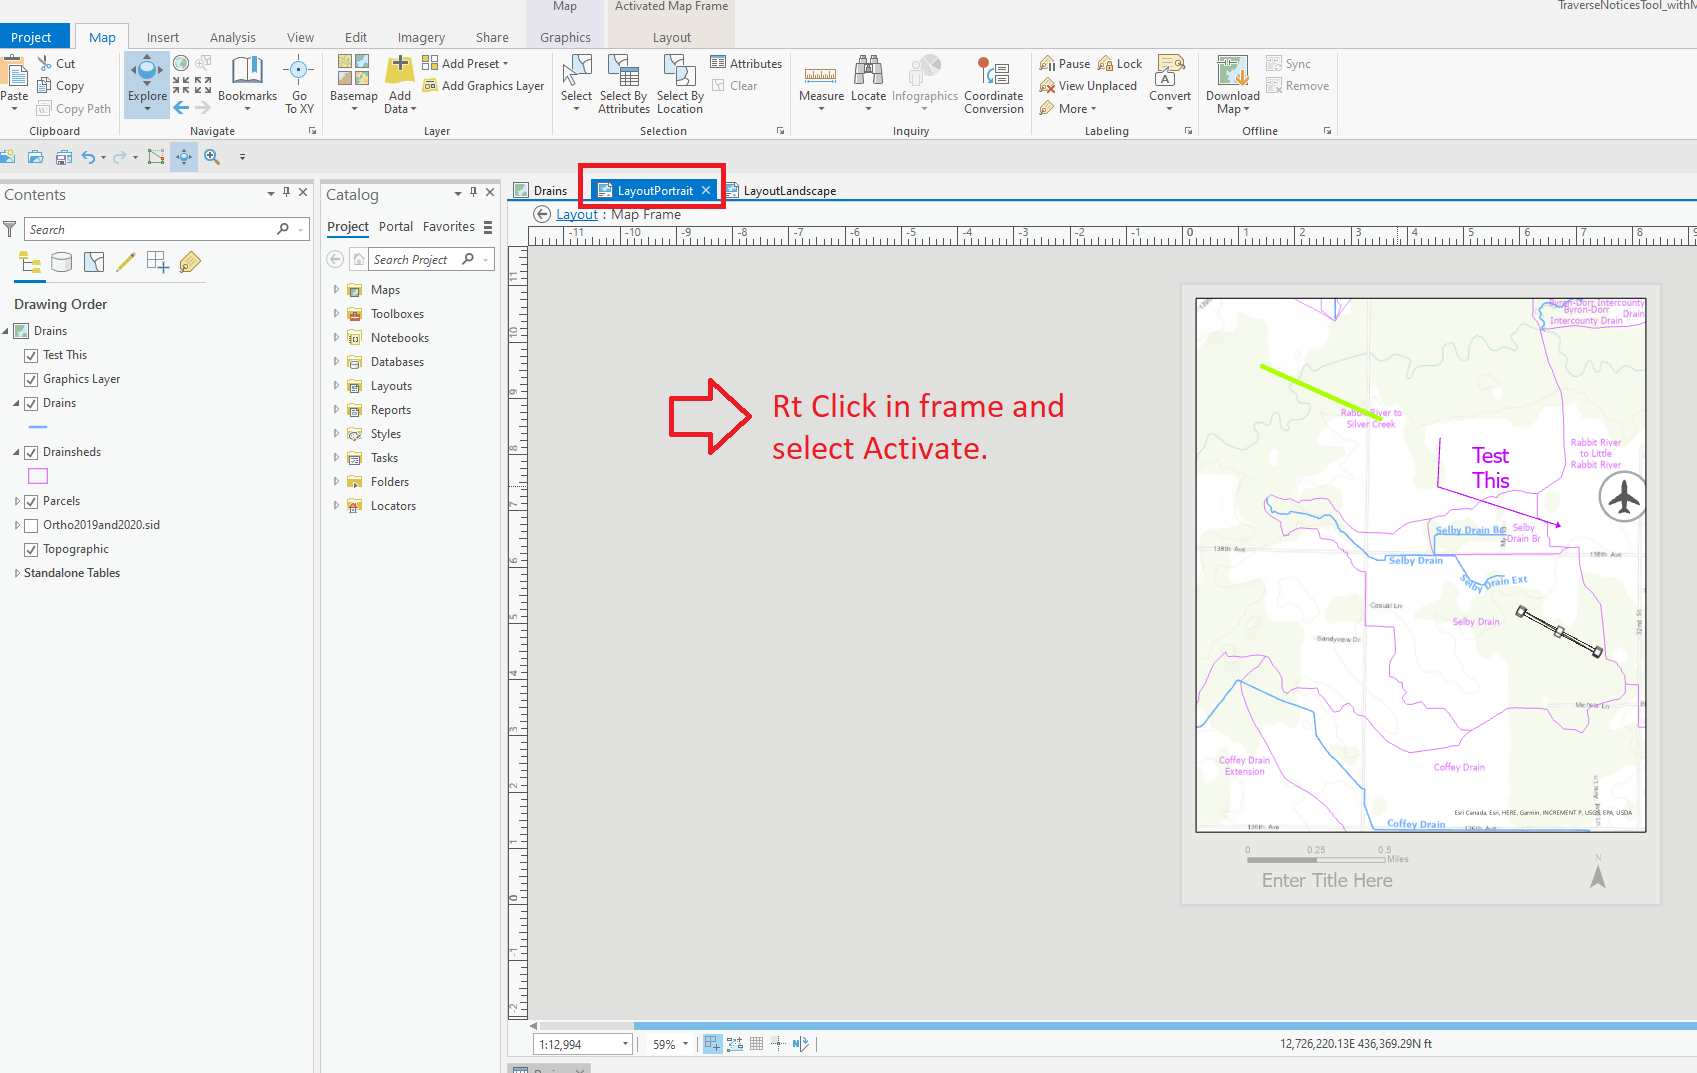
\includegraphics[width=.8\textwidth]{19SelectLayoutAndActivate.PNG}
 \caption{Activate Layout}


 \end{figure}  

\noindent {\btn {Right click in the layout choose \fbox{Pan (or zoom) to selected}}}

\vspace{.25in}

\noindent {\btn {To pan, hold left click and roll the mouse wheel to zoom }}


\clearpage

\paragraph{Using Map Graphic Elements}

\subparagraph{Graphic Elements} 

\begin{itemize}

\item Can be used to add notes, text, arrows, etc to the map.  

\item Map graphics stay in geographic position.

\end{itemize}

\noindent To create graphic elements:

\noindent {\btn {click }\fbox{Graphics Layer} in Contents Pane}

\begin{figure}[h!]
 \centering
     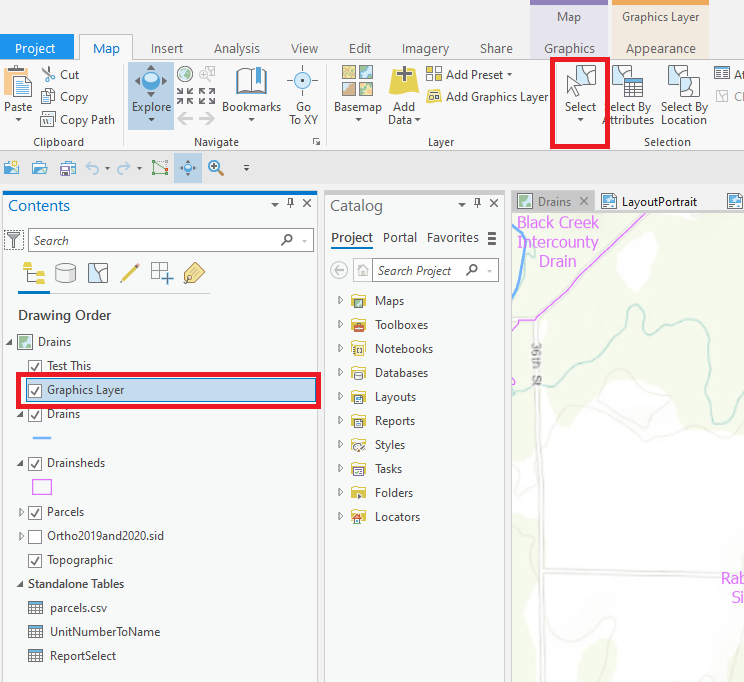
\includegraphics[width=.6\textwidth]{15sELECTEDgRAPHICSlAYERCapture.PNG}
 \caption{Click on Graphics Layer}

 \end{figure} 


\clearpage

\subparagraph{Set Target Graphics Layer}

To get to graphics options:

\noindent{\btn Map Tab {\lookArrow} \fbox{Graphics}}

\noindent {\btn set \fbox{Target Layer} to Graphics Layer}

 
\begin{figure}[h!]
 \centering
     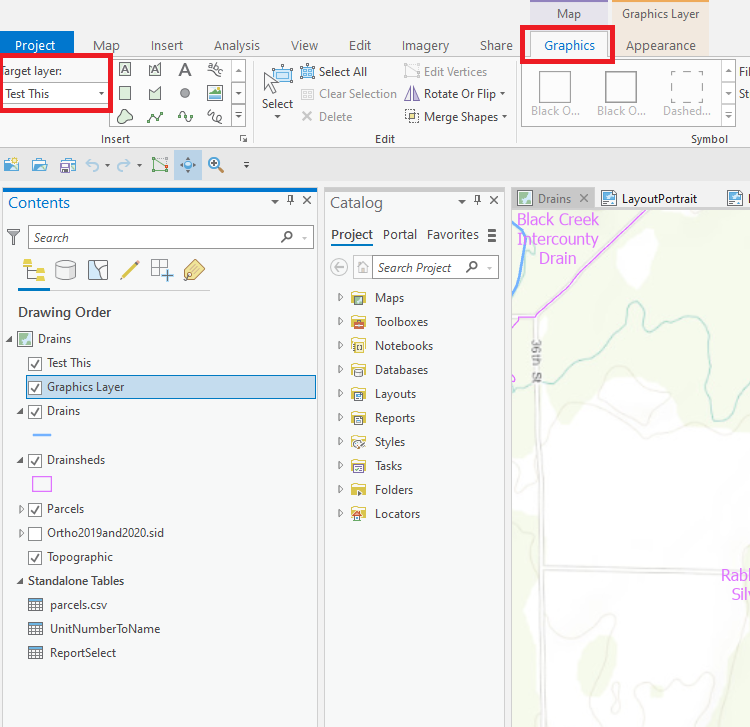
\includegraphics[width=.8\textwidth]{16ClickOnGraphicsTab.PNG}
 \caption{Graphics Tab}


 \end{figure} 


\clearpage

\subparagraph{Create a graphics element}


\noindent {\btn Select a graphics type}

\noindent Graphic types are chosen from this menu

 
\begin{figure}[h!]
 \centering
     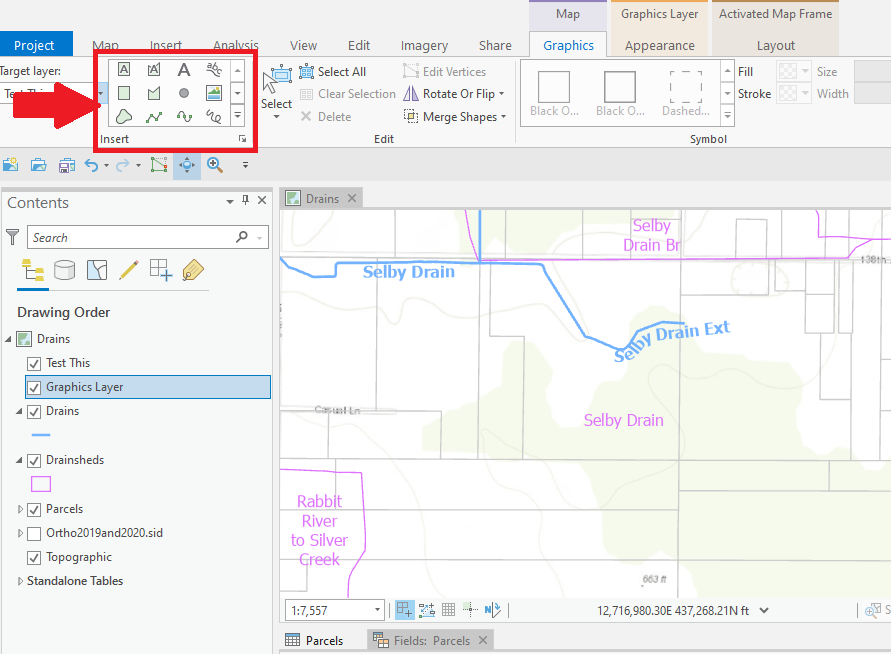
\includegraphics[width=.8\textwidth]{21GraphicsElement.PNG}
 \caption{Insert Graphic}


 \end{figure} 
\clearpage

\subparagraph{Using graphics from the Symbol Gallery}

\noindent Select any graphic element to change its style.

\noindent {\btn {Premade symbols can be accessed in the Symbol Gallery}}

\begin{figure}[h!]
 \centering
     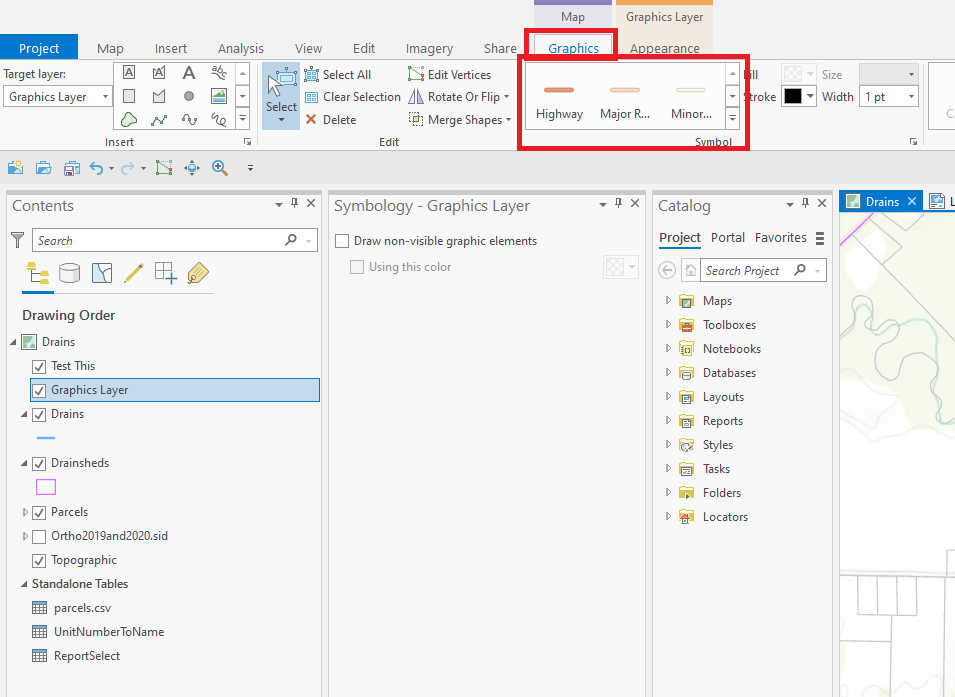
\includegraphics[width=.6\textwidth]{17GraphicsSymbolsAvailable.PNG}
 \caption{Symbol Gallery}


 \end{figure} 



\clearpage


\subparagraph{Custom Graphics}
Format the Selected Graphic as desired  


\begin{figure}[h!]
 \centering
     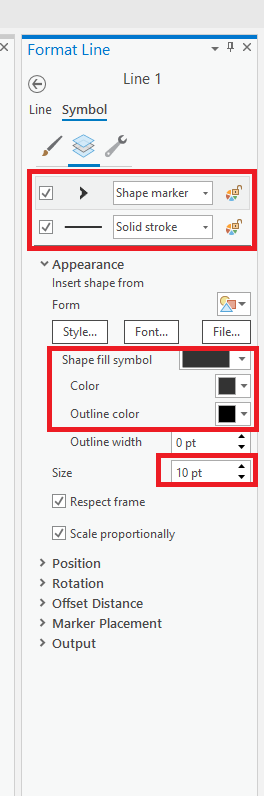
\includegraphics[width=.25\textwidth]{18FormatSymbol.PNG}
 \caption{Format Symbol}


 \end{figure} 



\clearpage




\subparagraph{Deactivate Layout Frame}

To go back to editing the map frame, deactivate the Layout frame


\noindent {\btn {Click }\fbox{Arrow}}

\begin{figure}[h!]
 \centering
     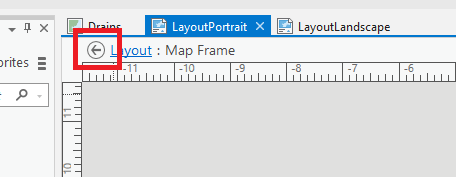
\includegraphics[width=.3\textwidth]{20CloseActivatedLayout.PNG}
 \caption{Deactivate}


 \end{figure} 

\clearpage


\subparagraph{Turning labels on and off}

In the Contents Pane, Right Click on the layer

\begin{itemize}

\item Select Label to turn labels on

\item Select Label again to turn labels off

\item Labels can be customized in Labeling Properties

\end{itemize}


\begin{figure}[h!]
 \centering
     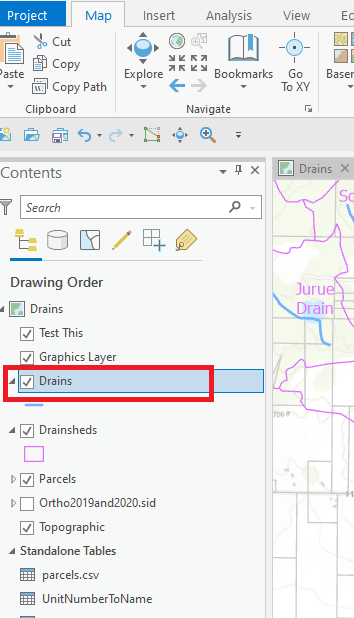
\includegraphics[width=.5\textwidth]{22LabelsOnOff.PNG}
 \caption{Labels On and Off}

 \end{figure}
 

\end{document}

